\documentclass{article}
\usepackage[utf8]{inputenc}
\usepackage{tikz}
\usetikzlibrary{patterns}

\begin{document}
\begin{titlepage}
   \begin{center}
       \vspace*{1cm}

       \textbf{Représentation fonctionnelle de diagrammes de Venn de dimension arbitraire.}

       \vspace{0.5cm}
        Outils pour le calcul des prédicats
            
       \vspace{1.5cm}

       \textbf{HANNIZ Anis, BEN HAMMOU Eddine}

       \vfill
            
       \vspace{0.8cm}
     
       \includegraphics[width=0.5\textwidth]{rouen}
            
   \end{center}
\end{titlepage}
\title{Rapport du Projet : Représentation fonctionnelle de
diagrammes de Venn de dimension arbitraire.}
\date{31 Décembre 2023}

\maketitle
\renewcommand{\contentsname}{Contenu}
\tableofcontents
\newpage
\section{Introduction}
	
Nous avons étudié les représentations graphiques des diagrammes de Venn à deux et trois dimensions, définis respectivement sur deux ou trois prédicats. Traditionnellement, ces prédicats sont représentés sous forme de cercles. Cependant, représenter ces diagrammes pour des dimensions plus élevées peut devenir complexe. Une alternative consiste à les interpréter comme des fonctions partielles reliant les zones du diagramme à un ensemble de contraintes de remplissage.
\\\\
Ce rapport offre une analyse détaillée des fonctions spécifiques implémentées dans le code Ocaml, explorant les concepts fondamentaux de la logique propositionnelle et des syllogismes. Il répond également aux questions énoncées, offrant une compréhension claire et détaillée des mécanismes sous-jacents et des méthodologies appliquées dans le cadre de la manipulation des diagrammes de Venn.
\\\\
La logique propositionnelle et les syllogismes font appel à des outils visuels tels que les diagrammes de Venn pour représenter et comprendre les relations entre ensembles et les implications logiques. Ce rapport s'attache à détailler les différentes étapes et procédures utilisées pour calculer les diagrammes de Venn associés à des formules syllogistiques, ainsi que pour déterminer la compatibilité entre ces diagrammes.
\\\\
En explorant les questions posées, ce rapport aborde en détail les concepts d'analyse des quantificateurs, d'utilisation des tables de vérité pour évaluer les formules logiques, et de construction des diagrammes de Venn correspondants. De plus, il détaille les étapes pour calculer la conjonction de deux diagrammes de Venn et explique comment déterminer la compatibilité de ces diagrammes en utilisant OCaml.
\\\\
En somme, ce rapport constitue une ressource complète et détaillée, offrant une compréhension approfondie des mécanismes fondamentaux des diagrammes de Venn dans le contexte de la logique propositionnelle et des syllogismes.

\newpage

\section{Définitions}

\subsection{\textbf{Diagramme de Venn}}
Un diagramme de Venn est une représentation graphique utilisée en théorie des ensembles et en logique pour illustrer les relations entre ensembles. Il est composé de formes géométriques, généralement des cercles, superposés ou juxtaposés, chacun représentant un ensemble. Les intersections et les unions des cercles permettent de visualiser les relations d'inclusion, d'intersection et d'union entre ces ensembles.


\subsection{\textbf{Opérations sur des diagrammes de Venn}}
Les opérations sur des diagrammes de Venn incluent des actions telles que la conjonction (intersection), la disjonction (union), la négation, la différence, et d'autres opérations logiques entre les ensembles représentés par les diagrammes de Venn. Ces opérations permettent de représenter graphiquement les résultats de différentes relations entre ensembles.


\subsection{\textbf{Logique propositionnelle}}
La logique propositionnelle est une branche de la logique formelle qui traite des propositions et de leurs relations en utilisant des connecteurs logiques tels que "et" ($\land$), "ou" ($\lor$), "non" ($\lnot$), "implication" ($\rightarrow$), etc. Elle étudie la structure des propositions indépendamment de leur signification spécifique, se concentrant sur la validité des arguments.
\\Cas de l'Implication
L'implication logique est une relation entre deux propositions, où une est la prémisse et l'autre est la conclusion. Si la prémisse est vraie, la conclusion doit également l'être.\\\\
Exemple : 
\begin{enumerate}
\item
\begin{center}
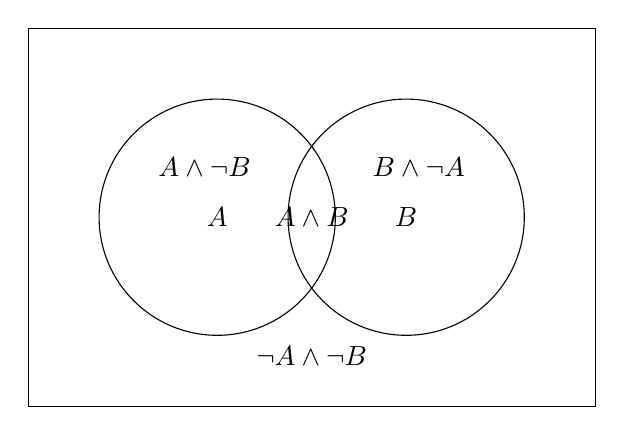
\begin{tikzpicture}[scale=1.6]
  \draw (-1.5,-1.5) rectangle (3,1.5);
  
  \node[circle, draw, minimum size=3cm] (A) at (0,0) {$A$};
  \node[circle, draw, minimum size=3cm] (B) at (1.5,0) {$B$};
  
  \node at (-0.1,0.4) {$A \land \lnot B$};
  \node at (1.6,0.4) {$B \land \lnot A$};
  
  \node at (0.75,0) {$A \land B$};
  \node at (0.75,-1.1) {$\lnot A \land \lnot B$};
  
\end{tikzpicture}
\end{center}
\newpage


\item
\textbf{Intersection (A $\cap$ B)}
\begin{center}
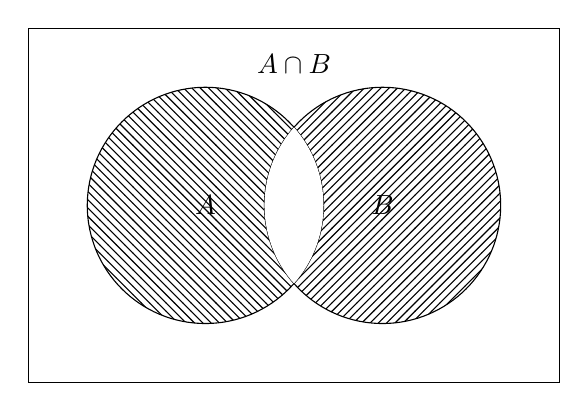
\begin{tikzpicture}[scale=1.5]
  \draw (-1.5,-1.5) rectangle (3,1.5);
  
  \node[circle, draw, minimum size=3cm, pattern=north west lines] (A) at (0,0) {$A$};
  \node[circle, draw, minimum size=3cm, pattern=north east lines] (B) at (1.5,0) {$B$};
  
  % Intersection sans hachure
  \begin{scope}
    \clip (A) circle (1cm);
    \fill[white] (B) circle (1cm);
  \end{scope}
  
  \node at (0.75,1.2) {$A \cap B$};
\end{tikzpicture}
\end{center}

\item
\textbf{Union (A $\cup$ B)}

\begin{center}
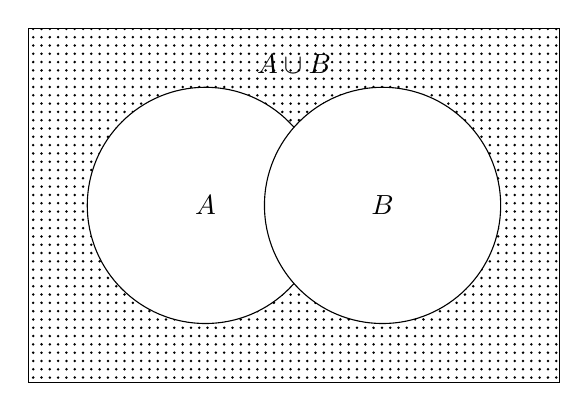
\begin{tikzpicture}[scale=1.5]
  \draw[pattern=dots]  (-1.5,-1.5) rectangle (3,1.5);
  
  \node[circle, draw, minimum size=3cm,fill=white] (A) at (0,0) {$A$};
  \node[circle, draw, minimum size=3cm,fill=white] (B) at (1.5,0) {$B$};
  
  \node at (0.75,1.2) {$A \cup B$};
\end{tikzpicture}
\end{center}

\item
\textbf{Différence (A $\setminus$ B)}

\begin{center}
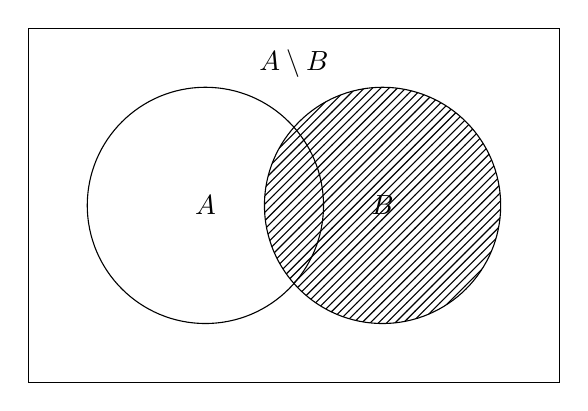
\begin{tikzpicture}[scale=1.5]
  \draw (-1.5,-1.5) rectangle (3,1.5);
  
  \node[circle, draw, minimum size=3cm] (A) at (0,0) {$A$};
  \node[circle, draw, minimum size=3cm, pattern = north east lines] (B) at (1.5,0) {$B$};
  
  \node at (0.75,1.2) {$A \setminus B$};
\end{tikzpicture}
\end{center}

\newpage
\item
\textbf{Complément (non A)}

\begin{center}
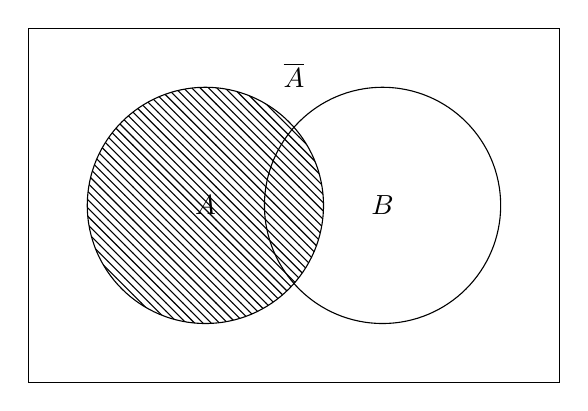
\begin{tikzpicture}[scale=1.5]
  \draw (-1.5,-1.5) rectangle (3,1.5);
  
  \node[circle, draw, minimum size=3cm, pattern=north west lines] (A) at (0,0) {$A$};
  \node[circle, draw, minimum size=3cm] (B) at (1.5,0) {$B$};
  
  \node at (0.75,1.1) {$\overline{A}$};
\end{tikzpicture}
\end{center}

\item
\textbf{Il existe A sans B}

\begin{center}
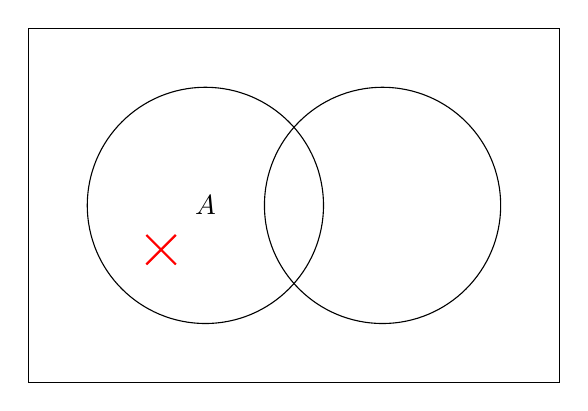
\begin{tikzpicture}[scale=1.5]
  \draw (-1.5,-1.5) rectangle (3,1.5);
  
  \node[circle, draw, minimum size=3cm] (A) at (0,0) {$A$};
  \node[circle, draw, minimum size=3cm] (B) at (1.5,0) {};
  
  
  % Croix dans A (à gauche)
  \draw[red, thick] (-0.5,-0.5) -- (-0.25,-0.25);
  \draw[red, thick] (-0.5,-0.25) -- (-0.25,-0.5);
\end{tikzpicture}
\end{center}

\item
\textbf{Il existe A qu'est B}

\begin{center}
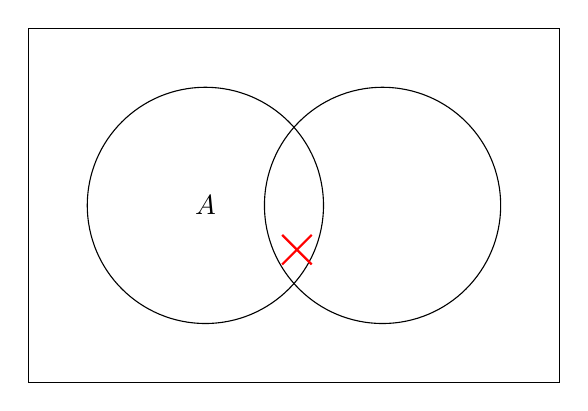
\begin{tikzpicture}[scale=1.5]
  \draw (-1.5,-1.5) rectangle (3,1.5);
  
  \node[circle, draw, minimum size=3cm] (A) at (0,0) {$A$};
  \node[circle, draw, minimum size=3cm] (B) at (1.5,0) {};
  
  
  % Croix dans A (à gauche)
  \draw[red, thick] (0.65,-0.5) -- (0.9,-0.25);
  \draw[red, thick] (0.9,-0.5) -- (0.65,-0.25);
\end{tikzpicture}
\end{center}

\end{enumerate}
\newpage
\subsection{\textbf{Syllogisme}}
Le syllogisme est un raisonnement déductif composé de deux propositions appelées prémisses et d'une conclusion. Il suit une structure logique particulière où une conclusion découle nécessairement des prémisses, basée sur des règles formelles. Il est souvent représenté sous forme de "Si A est vrai, et si A implique B, alors B est vrai".\\\\
Exemple : 
\begin{enumerate}
\item \textbf{Premisse 1 : A $\rightarrow$ B}
\item \textbf{Premisse 2 : B $\rightarrow$ C}\\\\

\begin{center}
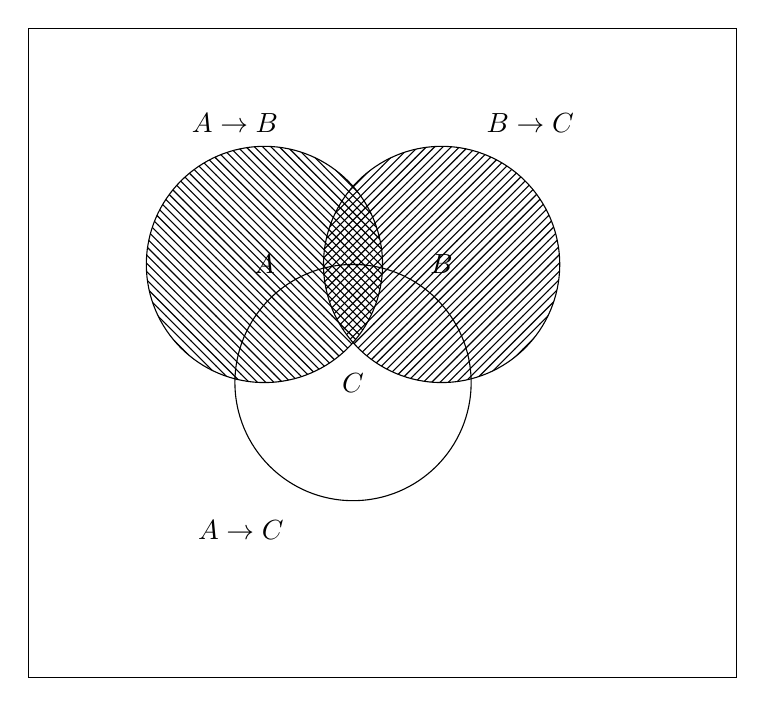
\begin{tikzpicture}[scale=1.5]
  \draw (-2,-1.5) rectangle (4,4);
  
  \node[circle, draw, minimum size=3cm, pattern=north west lines] (A) at (0,2) {$A$};
  \node[circle, draw, minimum size=3cm, pattern=north east lines] (B) at (1.5,2) {$B$};
  \node[circle, draw, minimum size=3cm] (C) at (0.75,1) {$C$};
  
  \node at (-0.25,3.2) {$A \rightarrow B$};
  \node at (2.25,3.2) {$B \rightarrow C$};
  \node at (-0.2,-0.25) {$A \rightarrow C$};
  
\end{tikzpicture}
\end{center}
\end{enumerate}
\newpage

\section{Code Ocaml}

\subsection{\textbf{Définition des types}}
\begin{itemize}
\item
\textbf{formule\_log\_prop} définit les différentes formes qu'une formule logique propositionnelle peut prendre en OCaml. Il inclut des variantes pour les atomes, les connecteurs logiques tels que "Et", "Ou", "Implication", "Non", etc., ainsi que des variantes pour des quantifications et des opérations sur des listes de formules.
\item
\textbf{formule\_syllogisme} représente les formules utilisées spécifiquement pour les syllogismes en OCaml. Il a deux variantes principales : \texttt{PourTout} et \texttt{IlExiste}, correspondant aux quantificateurs universel et existentiel respectivement, chacun prenant une formule logique propositionnelle.
\end{itemize}

\subsection{\textbf{Formule\_Log\_Prop.ml}}
Définit le type des formules de la logique propositionnelle. Il comporte des variantes pour les formules de base comme les atomes, les connecteurs logiques tels que Et, Ou, Non, etc., ainsi que des variantes pour des quantifications et des opérations sur des listes de formules.

\begin{itemize}
\item
\texttt{atome\_dans\_f} : \texttt{formule\_log\_prop -> string list}\\
- Renvoie une liste de chaînes de caractères correspondant à tous les atomes présents dans la formule.

\item
\texttt{est\_dans\_liste} : \texttt{string list -> string -> bool}\\
- Vérifie si une chaîne de caractères est présente dans une liste de chaînes.

\item
\texttt{fusion\_liste} : \texttt{string list -> string list -> string list}\\
- Fusionne deux listes en ajoutant à la deuxième liste tous les éléments de la première liste qui ne sont pas déjà présents dans la deuxième liste.
\item
\texttt{eval\_Formule\_Log\_Prop} : \texttt{string list -> formule\_log\_prop -> bool}\\
- Évalue une formule logique propositionnelle en fonction d'une interprétation donnée par une liste de chaînes de caractères.

\item
\texttt{table\_verite} : \texttt{string list -> formule\_log\_prop -> (string list * bool) list}\\
- Renvoie la table de vérité d'une formule sur les atomes issus de la formule elle-même et de l'ensemble alpha (liste de chaînes de caractères).

\item
\texttt{string\_of\_formule\_log\_prop\_var} : \texttt{string -> formule\_log\_prop -> string}\\
- Convertit une formule en chaîne de caractères en représentant les formules comme des prédicats unaires appliqués sur des occurrences de la variable donnée.
\end{itemize}


\subsection{\textbf{Formule\_Syllogisme.ml}}
Définit le type des formules utilisées pour les syllogismes. Il comporte deux variantes : \texttt{PourTout} qui prend une \texttt{formule\_log\_prop} et \texttt{IlExiste} qui prend également une \texttt{formule\_log\_prop}.
\begin{itemize}
\item
\texttt{string\_of\_formule} : \texttt{formule\_syllogisme -> string}
\\
- Conversion d'une formule en chaîne de caractères en considérant des prédicats unaires appliqués sur des occurrences de la variable 's'.
\\
- Utilise la fonction \texttt{string\_of\_formule\_log\_prop\_var} pour effectuer la conversion en fonction du type de formule (\texttt{PourTout} ou \texttt{IlExiste}).
\\
- Renvoie une chaîne de caractères représentant la formule avec le quantificateur universel pour \texttt{PourTout} et le quantificateur existentiel pour \texttt{IlExiste}.
\end{itemize}

\subsection{\textbf{Test.ml}}
\begin{itemize}
    \item \texttt{string\_of\_diagrams\_list } : \\
    Cette fonction prend une liste de chaînes de caractères représentant des diagrammes et renvoie une chaîne contenant la représentation de chaque diagramme avec son numéro correspondant.
    
    \item \texttt{string\_of\_premises} : \\
    Cette fonction prend une liste de listes de chaînes de caractères représentant des diagrammes de prémisse et renvoie une chaîne contenant la représentation de chaque prémisse avec les représentations de ses diagrammes.
    
    \item \texttt{test} : \\
    Cette fonction prend une liste de formules de syllogisme \texttt{ps} et une formule de syllogisme \texttt{c}. Elle effectue plusieurs étapes :
        \begin{itemize}
            \item Obtient les atomes (\texttt{alpha}) présents dans les formules de \texttt{ps}.
            \item Génère les diagrammes (\texttt{dps}) pour chaque formule de \texttt{ps}.
            \item Convertit les représentations des diagrammes en chaînes de caractères (\texttt{str\_dps}).
            \item Génère la représentation en chaîne de caractères de la conclusion (\texttt{str\_dc}).
            \item Génère la représentation en chaîne de caractères des diagrammes de la combinaison (\texttt{comb}).
            \item Concatène toutes ces informations dans une chaîne \texttt{s}, puis l'affiche.
        \end{itemize}
\end{itemize}
\newpage

\subsection{\textbf{DiagVenn.ml}}

\begin{itemize}
\item
\texttt{string\_of\_diag} : \texttt{diagramme -> string} \\
Conversion d'un diagramme en une chaîne de caractères en représentant les ensembles de prédicats avec leur remplissage (\texttt{Vide} ou \texttt{NonVide}).
\item
\texttt{diag\_from\_formule} : \texttt{string list -> formule\_syllogisme -> diagramme list} \\
Utilise une table de vérité associée au diagramme et construit de ce dernier une formule sur les prédicats issus de la formule elle-même ou de l'ensemble alpha (liste de chaînes de caractères).
\item
\texttt{conj\_diag} : \texttt{diagramme -> diagramme -> diagramme option} \\
Calcul de la combinaison ou conjonction de deux diagrammes, renvoyant \texttt{None} en cas d'incompatibilité.
\item
\texttt{est\_compatible\_diag\_diag} : \texttt{diagramme -> diagramme -> bool} 
Test de compatibilité entre deux diagrammes issus d'une prémisse et d'une conclusion.
\item
\texttt{est\_compatible\_diag\_list} : \texttt{diagramme -> diagramme list -> bool} \\
Test de compatibilité entre un diagramme issu d'une prémisse et une liste de diagrammes issus d'une conclusion.
\item
\texttt{est\_compatible\_list\_list} : \texttt{diagramme list -> diagramme list -> bool} \\
Test de compatibilité entre plusieurs diagrammes issus de prémisses et une liste de diagrammes issus d'une conclusion.
\item
\texttt{atome\_dans\_formules} : \texttt{formule\_syllogisme list -> string list} \\
Liste des atomes présents dans une liste de formules de syllogisme.
\item
\texttt{fusion\_pourtout\_diag\_list} : \texttt{diagramme list -> diagramme} \\
Fusion des diagrammes représentant tous les éléments de la liste avec pour valeur "Vide".
\item
\texttt{combinaison} : \texttt{formule\_syllogisme list -> diagramme list} \\
Combinaison des diagrammes issus de plusieurs formules de syllogisme.
\item
\texttt{est\_compatible\_premisses\_conc} : \texttt{formule\_syllogisme list -> formule\_syllogisme -> bool} \\
Test de compatibilité entre une liste de prémisses et une conclusion.
\item
\texttt{temoin\_incompatibilite\_premisses\_conc\_opt} : \texttt{formule\_syllogisme list -> formule\_syllogisme -> diagramme option} \\
Identification d'un diagramme de combinaison de prémisses incompatible avec une conclusion s'il existe.
\item
\texttt{temoins\_incompatibilite\_premisses\_conc} : \texttt{formule\_syllogisme list -> formule\_syllogisme -> diagramme list} 
Récupération des diagrammes incompatibles de combinaison de prémisses avec une conclusion.
\end{itemize}
\newpage


\section{Réponse aux questions}

\subsection{\textbf{Comment calculer des diagrammes de Venn associés à une valeur f de type formule\_syllogisme?}}

\begin{enumerate}
    \item \textbf{Diagrammes de Venn fonctionnels :}
    \begin{itemize}
        \item Chaque diagramme de Venn fonctionnel représente un ensemble spécifique basé sur une condition logique ou une table de vérité.
    \end{itemize}

    \item \textbf{Intersection des ensembles :}
    \begin{itemize}
        \item Pour calculer la conjonction des diagrammes de Venn `A` et `B`, il faut trouver la zone où les deux diagrammes se chevauchent ou se croisent. Cette zone représente l'intersection des ensembles.
    \end{itemize}
    \item \textbf{Analyser le quantificateur :}
    \begin{itemize}
        \item Si \texttt{f} est de la forme \texttt{PourTout formule\_log\_prop}, cela signifie que pour chaque élément dans l'ensemble de valeurs de \texttt{formule\_log\_prop}, la formule doit être vraie.
        \item Si \texttt{f} est de la forme \texttt{IlExiste formule\_log\_prop}, cela signifie qu'il existe au moins un élément dans l'ensemble de valeurs de \texttt{formule\_log\_prop} pour lequel la formule est vraie.
    \end{itemize}
    \item \textbf{Utiliser la table de vérité :}
    \begin{itemize}
        \item La table de vérité associée à \texttt{f'} permet d'évaluer la véracité de \texttt{f'} pour différentes combinaisons de valeurs de ses atomes. Chaque ligne de la table de vérité représente une telle combinaison.
    \end{itemize}

    \item \textbf{Interpréter la table de vérité pour les diagrammes de Venn :}
    \begin{itemize}
        \item Si \texttt{f} utilise le quantificateur \texttt{PourTout}, alors tous les atomes qui satisfont \texttt{f'} doivent être inclus dans le diagramme de Venn associé à \texttt{f}.
        \item Si \texttt{f} utilise le quantificateur \texttt{IlExiste}, alors au moins un atome satisfaisant \texttt{f'} doit être inclus dans le diagramme de Venn associé à \texttt{f}.
    \end{itemize}

    \item \textbf{Construction des diagrammes de Venn :}
    \begin{itemize}
        \item Les ensembles représentés dans les diagrammes de Venn sont définis par les valeurs de vérité de \texttt{f'} pour différentes combinaisons d'atomes.
        \item Chaque ensemble dans le diagramme de Venn peut être construit en fonction de la table de vérité. Les ensembles sont représentés par des zones qui sont vides ou non vides, selon les valeurs de vérité de \texttt{f'} pour différentes combinaisons d'atomes.
    \end{itemize}
\end{enumerate}

\newpage
\subsection{\textbf{Comment calculer la conjonction de deux diagrammes de Venn?}}
Nous allons utiliser la fonction "conj\_diag" qui est chargée de calculer la conjonction de deux diagrammes de Venn. Voici comment elle fonctionne :\\

\textbf{Comparaison des éléments dans les deux diagrammes:} Chaque élément (ensemble) dans le premier diagramme est comparé à son équivalent (s'il existe) dans le deuxième diagramme.\\

\textbf{Vérification de la compatibilité:} Si un élément existe dans les deux diagrammes, on compare les valeurs associées à ces éléments dans les diagrammes. Les valeurs sont Vide ou NonVide. Si les deux diagrammes définissent la même zone comme vide (Vide) ou non vide (NonVide), alors cette zone peut être présente dans le résultat de la conjonction. Si, cependant, une zone est définie comme vide (Vide) dans l'un des diagrammes et non vide (NonVide) dans l'autre, cela crée une incompatibilité, car les contraintes sont contradictoires.\\

\textbf{Résultat:} Si aucune incompatibilité n'est détectée pendant cette comparaison, un nouveau diagramme est créé, contenant les zones compatibles définies par les deux diagrammes d'origine. Sinon, si une incompatibilité est rencontrée, la fonction renvoie \texttt{None} pour indiquer que la conjonction est impossible en raison de contraintes contradictoires.\\

\textbf{Exemple :}\\
\textbf{Diagramme 1 (\texttt{d1}):}

\quad Zone A : NonVide

\quad Zone B : Vide

\quad Zone C : NonVide
\\
\textbf{Diagramme 2 (\texttt{d2}):}

\quad Zone A : Vide

\quad Zone B : NonVide

\quad Zone C : NonVide\\


\begin{center}
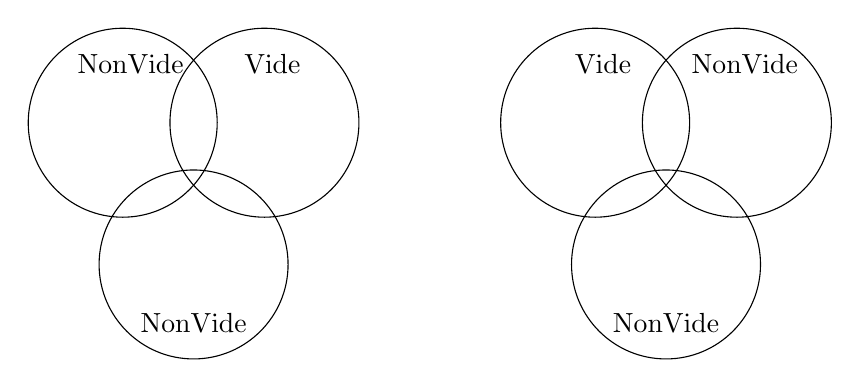
\begin{tikzpicture}[scale=1.2]
  % Diagramme 1
  \draw (-1,0) circle (1cm) node[above,shift={(0.1cm,0.5cm)}] {NonVide};
  \draw (0.5,0) circle (1cm) node[above,shift={(0.1cm,0.5cm)}] {Vide};
  \draw (-0.25,-1.5) circle (1cm) node[below,shift={(0cm,-0.5cm)}] {NonVide};
  
  % Diagramme 2
  \begin{scope}[xshift=5cm]
    \draw (-1,0) circle (1cm) node[above,shift={(0.1cm,0.5cm)}] {Vide};
    \draw (0.5,0) circle (1cm) node[above,shift={(0.1cm,0.5cm)}] {NonVide};
    \draw (-0.25,-1.5) circle (1cm) node[below,shift={(0cm,-0.5cm)}] {NonVide};
  \end{scope}
  
\end{tikzpicture}
\end{center}
\newpage

Lorsqu'on appele la fonction \texttt{conj\_diag d1 d2}, elle parcourt les zones correspondantes dans les deux diagrammes pour créer un nouveau diagramme résultant de la conjonction.

Voici comment cela se passerait :

\quad La fonction commence par examiner la zone A.

\quad Dans \texttt{d1}, la zone A est non vide.

\quad Dans \texttt{d2}, la zone A est vide.

\quad Comme ces deux diagrammes définissent des états différents pour la même zone, la conjonction est impossible. \\\\

\begin{center}
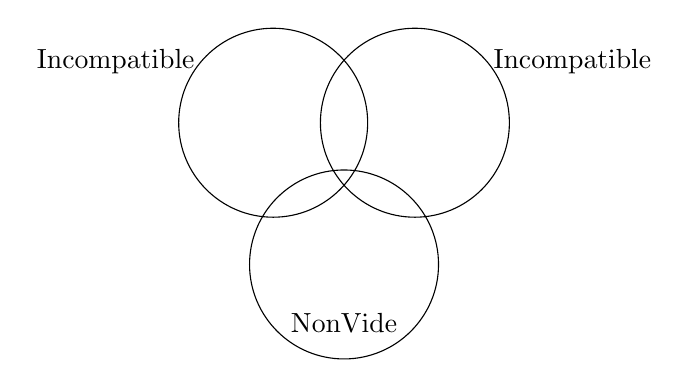
\begin{tikzpicture}[scale=1.2]
  % Conjonction
  \begin{scope}[yshift=-5cm,xshift= 2.5cm]
    \draw (-1,0) circle (1cm) node[above,shift={(-2cm,0.5cm)}] {Incompatible};
    \draw (0.5,0) circle (1cm) node[above,shift={(2cm,0.5cm)}] {Incompatible};
    \draw (-0.25,-1.5) circle (1cm) node[below,shift={(0cm,-0.5cm)}] {NonVide};
  \end{scope}
\end{tikzpicture}
\end{center}
La fonction renvoie \texttt{None}.
\newpage
\subsection{\textbf{Comment déterminer la compatibilité de deux diagrammes?}}


\textbf{Création des Diagrammes de Venn :}

Les formules logiques sont converties en ensembles de prédicats représentés sous forme de diagrammes de Venn. Chaque prédicat est associé à un ensemble dans le diagramme, soit "Vide" s'il est exclu, soit "NonVide" s'il est inclus.\\

\textbf{Conjonction de Diagrammes :}

Comme expliqué précedemment, la fonction \texttt{conj\_diag} calcule la conjonction de deux diagrammes de Venn, représentant une combinaison logique. Elle vérifie la compatibilité des ensembles entre les deux diagrammes pour déterminer la conjonction, renvoyant \texttt{None} en cas d'incompatibilité.\\

\textbf{Vérification de la Compatibilité :}

La fonction \texttt{est\_compatible\_diag\_diag} vérifie la compatibilité entre deux diagrammes spécifiques. \texttt{est\_compatible\_diag\_list} teste la compatibilité d'un diagramme avec une liste de diagrammes. \texttt{est\_compatible\_list\_list} vérifie si chaque diagramme d'une liste est compatible avec au moins un diagramme d'une autre liste.\\

\textbf{Illustration de l'Asymétrie de la Compatibilité :}

Considérons deux ensembles :\\
A représente l'ensemble des nombres premiers.\\
B représente l'ensemble des nombres impairs.

\begin{center}
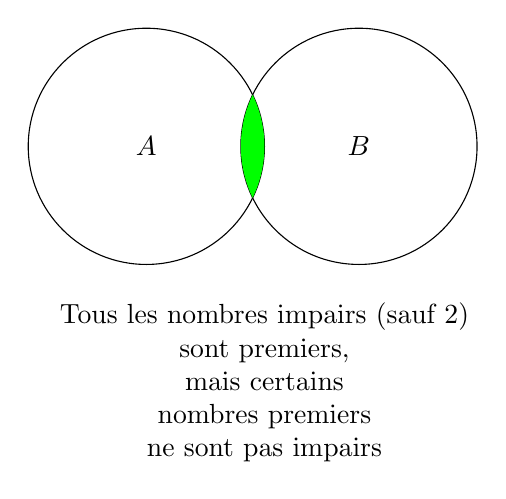
\begin{tikzpicture}[scale=1.5]
  % Ensemble A : Nombres premiers
  \node[circle, draw, minimum size=3cm] (A) at (0,0) {$A$};
  
  % Ensemble B : Nombres impairs
  \node[circle, draw, minimum size=3cm] (B) at (1.8,0) {$B$};
  
  % Zone où B est inclus dans A
  \begin{scope}
    \clip (A) circle (1cm);
    \fill[green] (B) circle (1cm);
  \end{scope}
  
  % Texte indiquant l'inclusion asymétrique
  \node[align=center] at (1,-2) {Tous les nombres impairs (sauf 2)\\ sont premiers,\\ mais certains\\ nombres premiers\\ ne sont pas impairs};
\end{tikzpicture}
\end{center}
Dans cette illustration, la zone verte représente l'ensemble des nombres impairs inclus dans l'ensemble des nombres premiers. Cela démontre que tous les nombres impairs (à l'exception de 2) sont inclus dans l'ensemble des nombres premiers, tandis qu'il existe des nombres premiers qui ne sont pas impairs, illustrant ainsi l'asymétrie de la relation entre les deux ensembles.
\newpage

\section{Conclusion}

Ce rapport a exploré en détail les fondements et les applications des diagrammes de Venn dans le cadre de la logique propositionnelle et des syllogismes. En plongeant dans les concepts d'analyse des quantificateurs, de manipulation des tables de vérité, de construction et de manipulation des diagrammes de Venn, il a offert une perspective approfondie sur ces outils visuels cruciaux.\\

Les fonctions implantées dans ce projet en OCaml ont concrétisé ces concepts en offrant des méthodes pour représenter, calculer et évaluer des diagrammes de Venn associés à des formules logiques ou des syllogismes. Ces outils ont permis la création de tables de vérité, la conjonction de diagrammes, ainsi que la détermination de la compatibilité entre eux.\\

Ainsi, ce rapport constitue une ressource complète pour appréhender les mécanismes sous-jacents à la représentation visuelle des relations entre ensembles. Il propose une vision claire sur l'utilisation des diagrammes de Venn dans le contexte de la logique formelle. Les explications détaillées, accompagnées d'exemples concrets, et la description des fonctions implémentées, fournissent une base solide pour l'application et la poursuite de l'exploration de ces concepts.\\

En définitive, ce rapport ouvre la voie à une utilisation plus avancée des diagrammes de Venn dans la logique formelle et offre un point de départ solide pour des recherches ultérieures et des applications pratiques dans ce domaine.

\end{document}
